\documentclass[aspectratio=169]{beamer}
\hypersetup{pdfpagemode=FullScreen}
\usetheme[progressbar=frametitle]{metropolis}
\usepackage{appendixnumberbeamer}
\usepackage{listings}
\bibliographystyle{plainnat}
\usepackage{hyperref}
\usepackage{booktabs}
\usepackage[backend=biber]{biblatex}
\addbibresource{references.bib}
\usepackage[scale=1]{ccicons}
\usepackage{subfig}
% \usepackage{enumitem} % not compatible with enumerate in beamer class
\usepackage{xspace}
\newcommand{\themename}{\textbf{\textsc{metropolis}}\xspace}

\graphicspath{ {./img/} }

\title{HB+Trie}
% \subtitle{Subtítulo}
% \date{\today}
\date{June 02, 2022}
\author{Thushjandan \& François-Xavier}
\institute{Data Management Data Structures}

\begin{document}

\maketitle

\begin{frame}{Agenda}
    \setbeamertemplate{section in toc}[sections numbered]
    \tableofcontents
\end{frame}
\section{Motivations}
\begin{frame}[t]
    \frametitle{Motivations}
       Variable-length sized keys
    
    Disadvantages with B+ tree or LSM-tree:
    \begin{itemize}
    	\item Fanout degree decreases if key length increases
    	\item Tree Height grows to maintain the same capacity
    	\item Benefit of prefix B+ tree becomes limited for randomly distributed keys
    	\item B+ tree nodes are randomly scattered on disk when it ages 
    \end{itemize}
\end{frame}
\section{Overview}
\begin{frame}[t]
    \frametitle{Overview}
    HB+ trie stands for \textit{Hierarchical B+ tree based trie}
    
    Characteristics:
    \begin{itemize}
    	\item Key space is divided into buckets. Every bucket has its own HB+ trie
    	\item High disk throughput due to append-only disk layout
    	\item Disk updates are delayed with a \textbf{Write buffer index}
    \end{itemize}
\end{frame}
\begin{frame}[t]
	\frametitle{Overview}
	\begin{figure}[h!]
		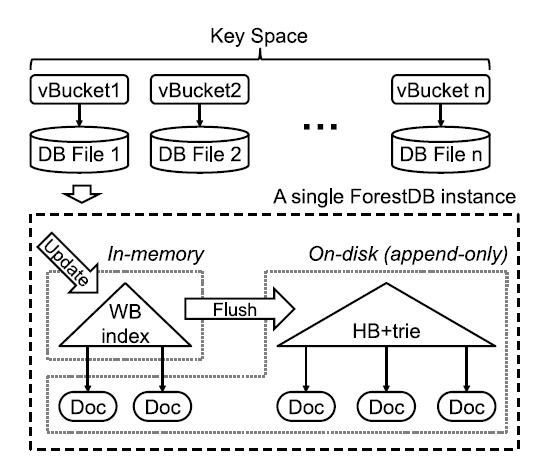
\includegraphics[scale=0.5]{architecture}
		\caption{Architecture}
	\end{figure}
	\centering
\end{frame}
\begin{frame}[t]
	\frametitle{Overview}
	HB+ trie stands for \textit{Hierarchical B+ tree based trie}
	
	Characteristics:
	\begin{itemize}
		\item Key space is divided into buckets. Every bucket has its own HB+ trie
		\item High disk throughput due to append-only disk layout
		\item Disk updates are delayed with a \textbf{Write buffer index}
		\item Fixed size chunking of the key
		\item Every unique chunk has a dedicated B+ tree
	\end{itemize}	
\end{frame}
\begin{frame}[t]
	\frametitle{Overview}
	\begin{figure}[h!]
		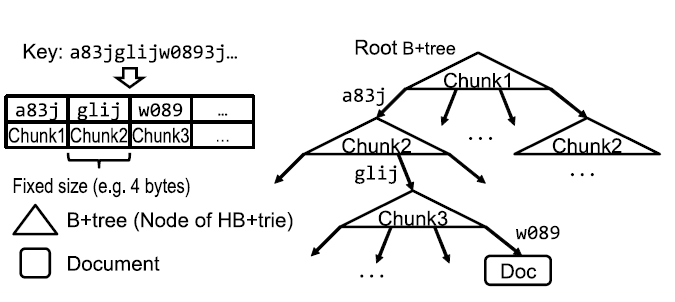
\includegraphics[scale=0.7]{logical_layout}
		\caption{Chunking}
	\end{figure}
	\centering	
\end{frame}
\begin{frame}[t]
	\frametitle{Overview}
	\begin{figure}[h!]
		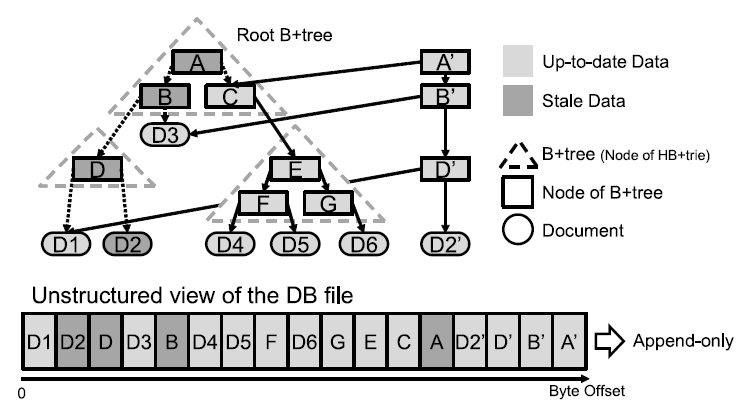
\includegraphics[scale=0.5]{disk_layout}
		\caption{Disk layout}
	\end{figure}
	\centering	
\end{frame}
\section{Implementation}
\begin{frame}[t]
    \frametitle{Implementation}
    \begin{itemize}
    	\item Using 16 byte chunks for keys
    	\item Each page frame holds a complete B+ subtree.
    	\item Storing pageId in the leaf to reference a B+ subtree
    \end{itemize}
\end{frame}
\begin{frame}[t]
	\frametitle{Implementation - Chunking}
	\begin{figure}[h!]
		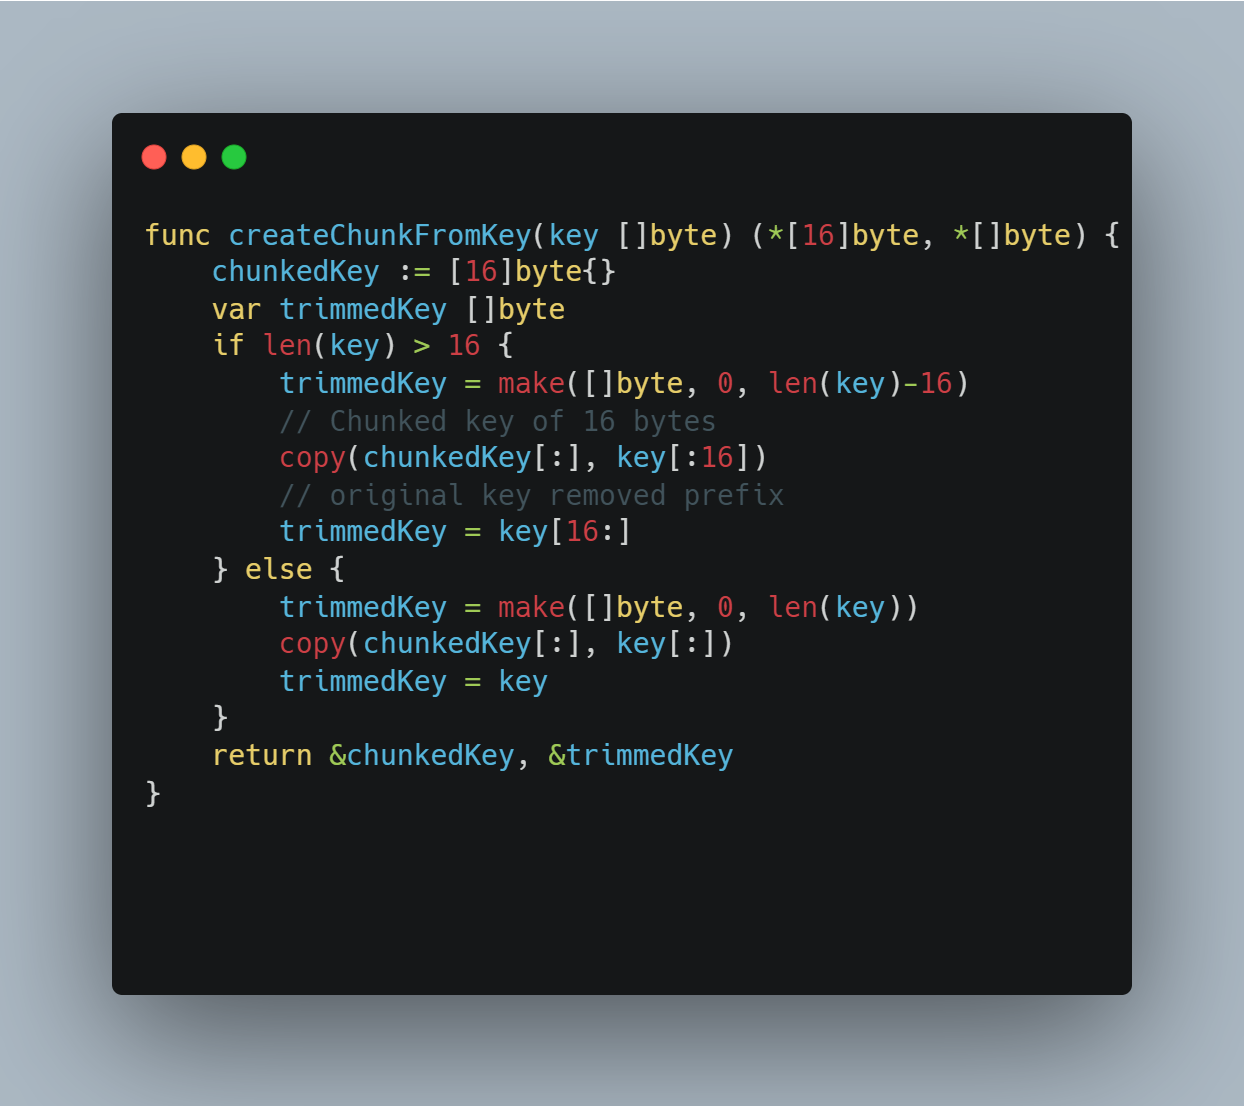
\includegraphics[scale=0.19]{code_chunking}
	\end{figure}
	\centering
\end{frame}
\begin{frame}[t]
	\frametitle{Implementation - Insert}
	\begin{figure}[h!]
		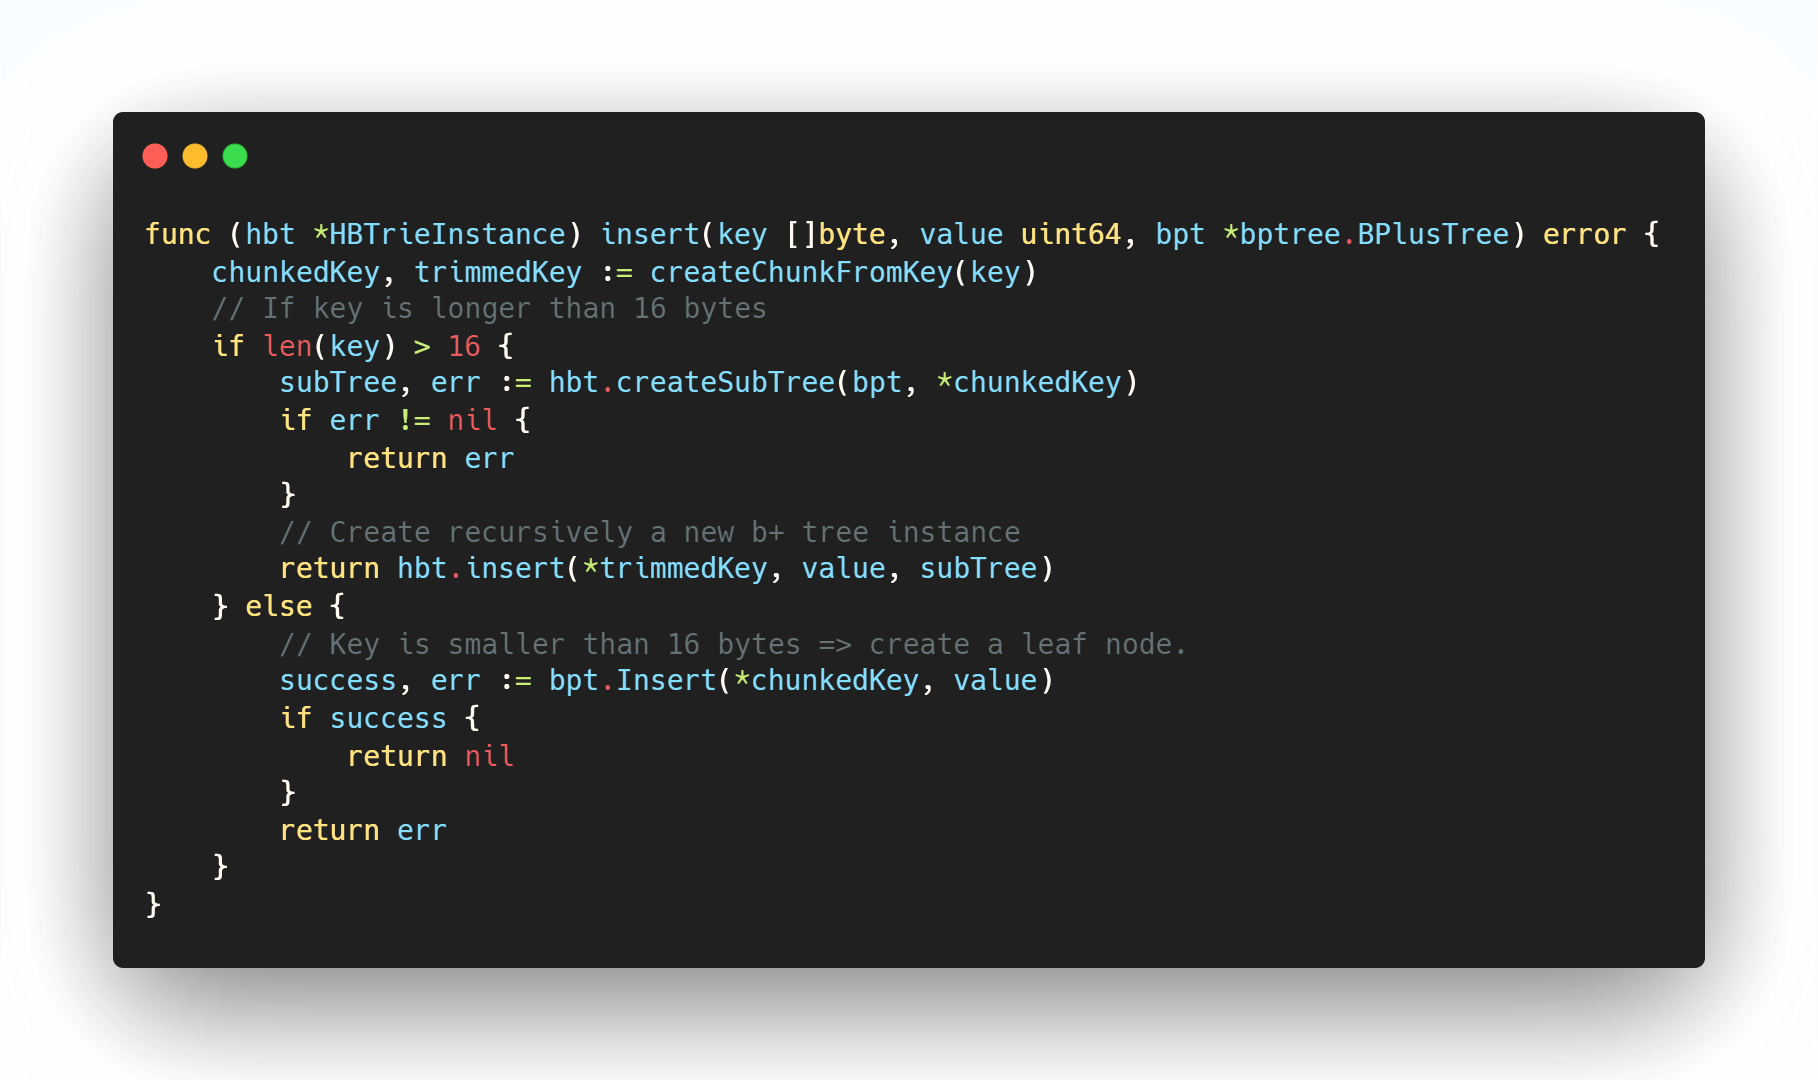
\includegraphics[scale=0.19]{code_insert}
	\end{figure}
	\centering
\end{frame}
\begin{frame}[t]
	\frametitle{Implementation - Search}
	\begin{figure}[h!]
		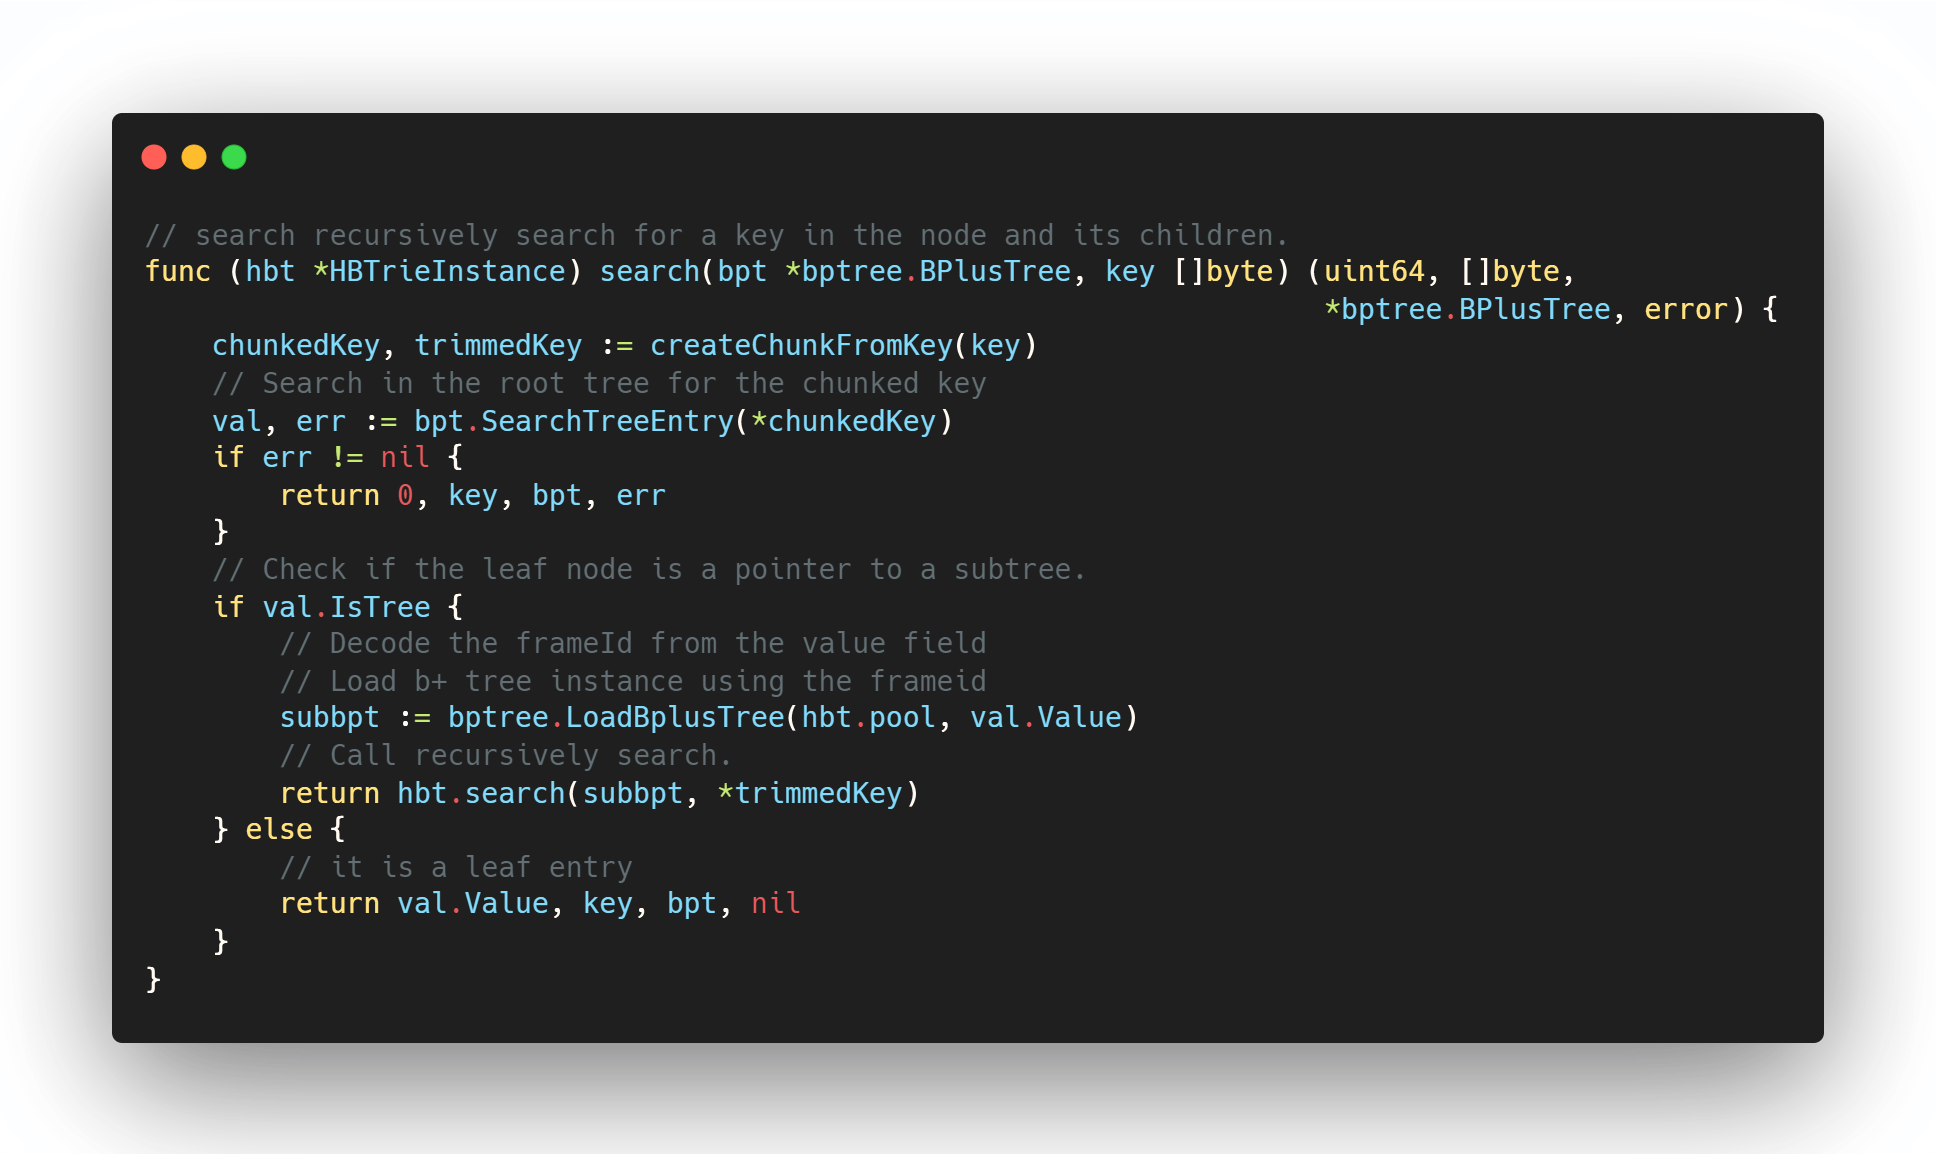
\includegraphics[scale=0.18]{code_search}
	\end{figure}
	\centering
\end{frame}
\begin{frame}[t]
	\frametitle{Implementation - Page frame}
	\begin{figure}[h!]
		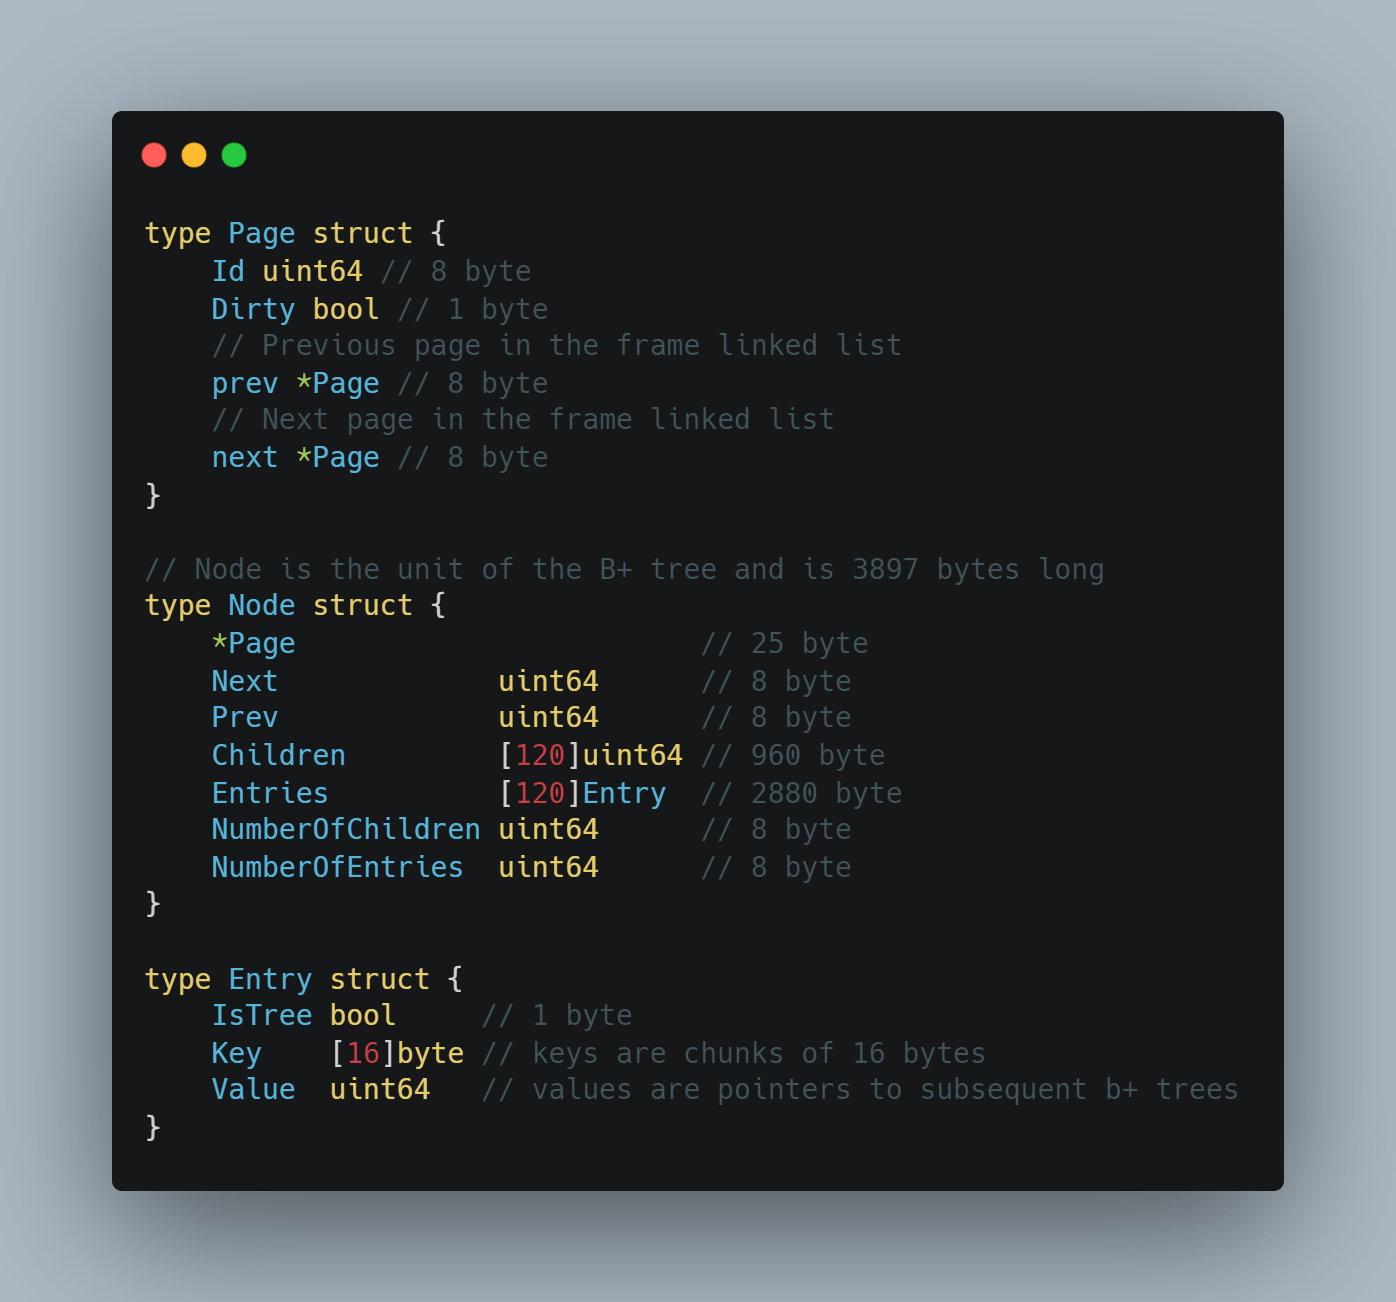
\includegraphics[scale=0.16]{code_page}
	\end{figure}
	\centering
\end{frame}
\section{Performance}
\begin{frame}[t]
    \frametitle{Performance}
    \begin{figure}[h!]
    	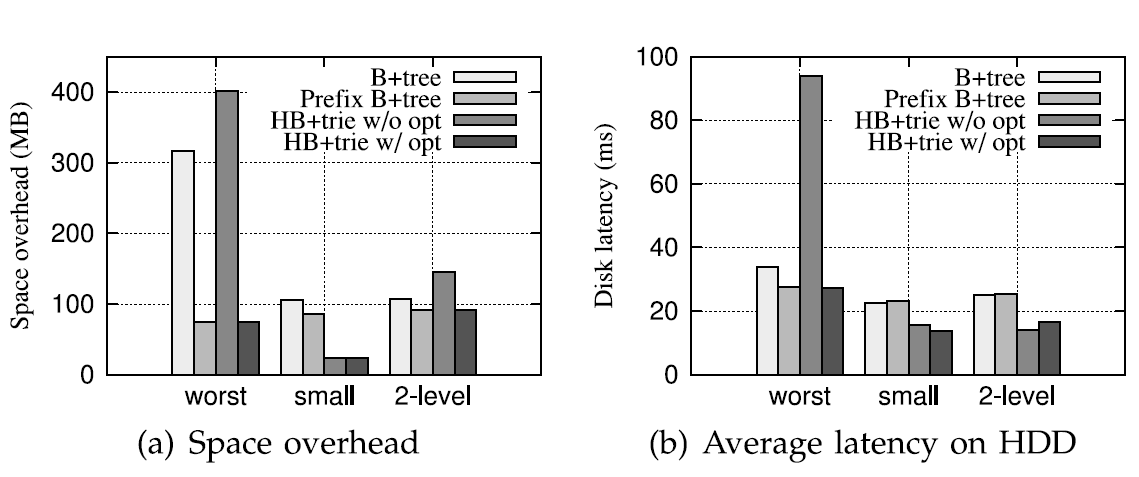
\includegraphics[scale=0.5]{comparision_bplus}
    \end{figure}
    \centering
\end{frame}
\section{Possible improvements}
\begin{frame}[t]
    \frametitle{Possible improvements}
    HB+ trie is not a balanced structure
    \begin{itemize}
    	\item Leads to key skew under specific key pattern
    \end{itemize}

	To address this issue, Leaf B+ tree extension is proposed
	\begin{figure}%
		\centering
		\subfloat[\centering Without extension]{{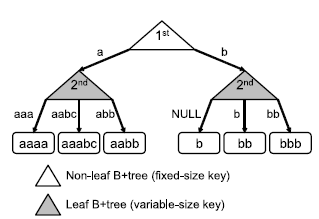
\includegraphics[scale=0.65]{skew_initialState} }}%
		\qquad
		\subfloat[\centering With extension]{{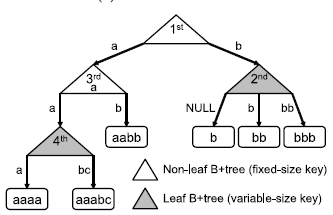
\includegraphics[scale=0.65]{skew_result} }}%
	\end{figure}
\end{frame}
\begin{frame}[t]
	\frametitle{Possible improvements}
	Performance of Range scans are bad in comparison with B+ tree.
	
	Write Buffer index improves the write throughput and lowers write amplifications
	
\end{frame}
\section{Discussion}
\end{document}
